\par\vspace{5mm}
{\large \textbf{Traffic Volume - Compare with Previous Day}}

When the user selects the **"Compare w/ Prev Day"**\colorbox{gray!20}{
\includegraphics[width=0.2\textwidth]{img/common/commonarea/results/CompareTheDaySmall.png}} option, the data displayed will include a comparison with the previous day's traffic data. This feature allows users to easily view how traffic has changed from one day to the next. The comparison is shown in terms of both the traffic volume and the percentage change.

As shown in the example below, users can see the differences in the traffic data for each operator. The data is displayed alongside arrows indicating whether the traffic has increased or decreased, along with the percentage change from the previous day.

\begin{figure}[ht]
  \centering
  \colorbox{gray!20}{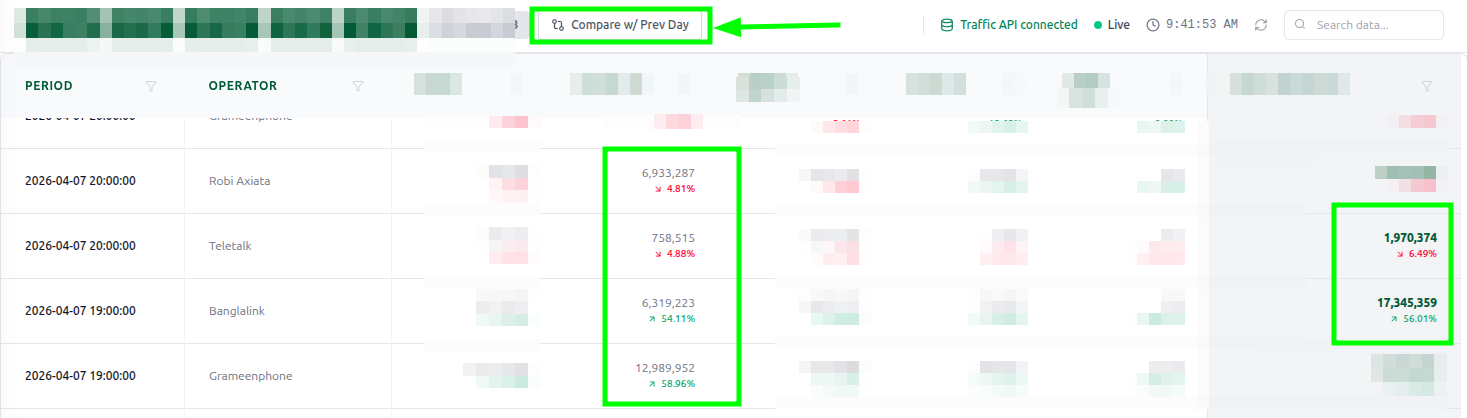
\includegraphics[width=.97\textwidth]{img/common/commonarea/results/CompareTheDay.png}}  % Replace with the path to your image file
  \caption{Example of Traffic Volume Comparison with Previous Day}
\end{figure}

This feature helps users quickly assess performance and identify trends in traffic over time.